%\documentclass{tufte-handout}
\documentclass{article}
\usepackage{amsmath,amsthm}
\usepackage{fontspec}
\usepackage{float}
%\usepackage{unicode-math}
%\setmathfont{Palatino Linotype}
%\setmainfont{Palatino Linotype}
%\usepackage{minted}
%\usemintedstyle{bw}
\usepackage{hyperref}

%\input{vc.tex}

%\newtheorem{claim}{Claim}[section]
\title{Control of Batch Tank using Raspberry Pi \\ FRTN01 project - Group 20}
%\date{\GITDate,\\\small\GITAbrHash}
\date{}
\author{Johan Anderholm \\ Jonathan Kämpe \\ Mikael Sahlström \\ Mikael Nilsson}

\begin{document}
\maketitle
\newpage
\tableofcontents
\newpage
\section{Problem description}
% An introduction that states the problem that has been solved.
This project aims to control a process called batchprocess that consists of a
batchtank, two pumps (one for pumping into the tank and one to pump out of the
tank), a heater, a cooler and a mixer. As stated in the project descriptions
\cite[p.~6]{project12}, we should simultaneously control the level and
temperature in the tank while simulating an exothermic chemical reaction.

This means that the heater will simulate the exothermic reaction and we'll use
the in pump to control the temperature. The out pump will then be used
to control the level which can be set dynamically in a settings file for the PID client that controls this pump.

There are sensors on the batchprocess that measures the water level and temperature.

\section{Program structure}
% A section describing the main program structure, both from a class
% and and a real-time perspective. If possible illustrate this with some
% type of figure.
This project is designed as a two-tier client/server system 
\cite[p.~6]{clientserver} where none of the control processes need to be directly
connected to the batch tank.

The server contains of a driver that communicates with the batch tank over a
serial interface and the server part of the server that receives connections from
clients and serves them with desired data and redirects control signals from
clients to the driver which sends them to the batch tank. The communication
between the server and its clients is done via the TCP/IP protocol which means
that the clients can be located anywhere. In our tests we have had clients
running on the same device as the server and on separate devices connected
through a switch and TP-cable.

\subsubsection{External libraries}
\begin{itemize}
\item{jQuery}
\item{Flot}
\end{itemize}

\subsubsection{Protocol Buffers}
The messages used to communicate between clients and the servers are
described using a interface description language called Protocol
buffers, or protobuf \cite{protobuf}.


\subsection{Server}
The server is implemented using C++ in order to run well on the Raspberry Pi as
there is currently not any acceptable JVM with proper JIT available. It
also makes calling timing functions more appropriate for real time tanks
considerably easier. The server consists of the following classes:

\begin{description}
\item[IORegistry]
  This class is used as an interface against the batchtank server.
  Mutexes are used in order to make reading and writing to the process
  atomic operations.

\item[ConnectionThread]
  Whenever a connection is made to the server a \verb+ConnectionThread+
  is fired and given control over that particular connection. Each
  connection contains a main reading loop executing controller events.
  It is running as a detached thread.

\item[PeriodicTask]
  Executes a function on a strictly regular basis. Uses
  \verb+clock_nanosleep+  with \verb+TIMER_ABSTIME+ and
  \verb+CLOCK_MONOTONIC+ and should have a fairly high resolution.

\item[Sampler]
  Ran as periodic task to sample at specified intervals.
\end{description}

\subsubsection{Use scenario}
The server listens to a port specified in a \verb+.ini+ file. When a client
connects the connection is assigned a dedicated \verb+ConnectionThread+. 
Upon a register event recieved a \verb+PeriodicTask+ is fired together
with a sampler that samples and sends samples to the client at a regular
interval. The register message contains data such as period time and
what sensors to read.

The client may respond with control signal events which specify what
value should be set as well as to what output. It also contains the
reference value used for this control signal.

Setting and getting values from the batch process is protected by a
\verb+IORegistry+ however locking of the registry is external, i.e. it
contains a public mutex and does no locking on its own. This is done in
order to enable batching several gets and sets as single atomic
operations. The \verb+IORegistry+ also contains copies of reference
values as well as control signals for plotting use cases.


\subsection{Driver}
The driver for the communication over a serial port is written in the C language.
It makes use of the Unix API for terminal I/O. The operative system's driver will
map the serial device to a file descriptor, hence the reads and writes are done
with standard C functions read(3), write(1), open(2) and close(2).  The serial
connection has a speed of 115200 baud. 

The driver has a set and get function and a couple of enumerators specifying the
sensor to set or to get. The driver supports all available sensors or motors of
the batch tank; temperature, water level, in/out pump, mixer, cooler and heater.

The get function is blocking with a timeout of 1 second. Any kind of failure will
make the functions return a negative number. Data is sent and received in chunks
of 8 bits. The get function sends a byte asking the batch tank to send some
information about a specific sensor or motor, it then blocks on the read function
until all bytes are read. The set function simply puts commands on the serial
line. The bytes are processed in accordance to the source code that runs on the
batch tank \cite[line 150-223]{kokare.c}. 

The driver will always parse the whole value into bytes and then send it to the
batch tank. The batch tank only supports values between 0 and 255. The
temperature and the water level sensors may gerenrate greater values than 255.
This is all supported. The driver is not thread safe.

The driver will always parse the whole value into bytes and then send it to the
batch tank. The batch tank only supports values between 0 and 255. The
temperature and the water level sensors may gerenrate greater values than 255.
This is all supported. The driver is not thread safe.

\subsection{PID client}
The PID client, written in C++, consists of a main method which uses boost libraries for communication with the server and a PID class. The PID class have these public members:
\begin{itemize}
\item{void updateParameters(const PIDParameters\&);}
\item{double next(double);}
\item{void updateStates();}
\end{itemize}

The PID parameters include K, Ti, Td, Tr, ref, umin, umax, inverted, and period.

\subsubsection{Use scenario}
The client starts with parsing server and controller details from a \verb+.ini+ file. After a succesful connection it sends sensor and period to the server and starts to wait for sensor values. When one is received a control signal is calculated and sent. Then controller states are updated and the client starts to wait for the next sensor value. The client also updates the PID parameters as they are changed in the \verb+.ini+ file.


\subsection{Plot client}
The plot client, written in Python \cite{python}, is in itself a server/client
system where the server is a client to the main server and the clients are web
browsers running the Javascript plotting code. When started, a HTTP server will
start serving a HTML and Javascript page which is to be run in a browser. This
page will request new data to plot from the HTTP server which then requests data
from the main server. The main server then sends data (such as water level,
control signals and reference signals) to the HTTP server which parses it into
JSON \cite{json} formatted data and sends it to the plot page. The data format is
as follows:
\begin{verbatim}
{"Plot name": { "Curve name": [y value, ...], ... }, ... }
\end{verbatim}
The data will be received and parsed by Javascript code which will go through it
step by step. First, the code checks if a plot exists and creates the plot if
not. Then if the curves exists in the plot and creates them if not. Then each y
value will be shifted onto the curve data, from the right. This data will
initially contain 100 zeros. The same amount of data that is shifted from the
right is shifted out from the left so that the curve always contains 100
data points. This will create an effect where the data flows from the right to
the left smoothly.

\section{Control design}
% A section describing the control design aspects of the p\ref{kokare.c}. roject.
The controller is a standard PID controller implemented with forward approximation integral, forward approximation derivative, bumpless transfer, and tracking as anti-windup.

The control loop does the following in one iteration.
\begin{itemize}
\item{Wait for y}
\item{Calculate u}
\item{Send u}
\item{Update states}
\end{itemize}


\section{Running the system}
% A section describing the user interface in the project including a short
% HowTo description on how to start and operate the program.
To start the system one should first connect a device to the batch tank and the
serial connection to a USB port using a serial to USB adapter. After connecting
the device to the batch tank start the server named batchtank\_server and it will
start listening for incoming TCP connections from clients. Run these on either
the same device as the server or on separate devices connected, via TCP/IP, to
the server.

\section{Results}
% A section containing the results. In case the project is a control-oriented
% project this should include plots of measurement signals, reference sig-
% nal, and control signal. If the project is more of a real-time nature then
% this section could contain measurement results of different type.
In all our tests we can see that the water level have a "high frequency" noise
that comes from when the water stream from the in pump hits the water in the
tank. This noise is reflected upon the control signals that are based on water
level measurements and can be seen in figure~\ref{fig:out pump}.

The high frequency noise does not affect the pumping power so much as they can not make such small and frequent changes in power.

Figure~\ref{fig:out pump} shows how a PID client controlling the out pump reacts
to a change in the in flow of water. The straight curve at 400 (y value) is the reference water level the out pump should hold, the top curve is the water level and the bottom curve is the control value which is sent to the out pump.
\begin{figure}[H]
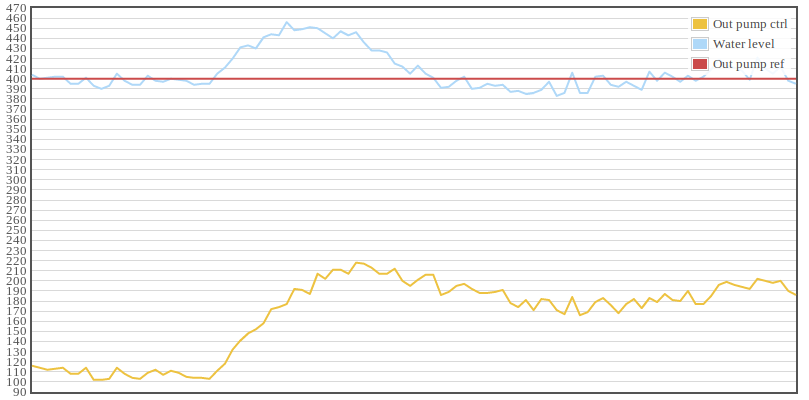
\includegraphics[width=1.0\textwidth]{plot1.png}
\caption{A PID client regulating the water level with the out pump with reference value 400.}
\label{fig:out pump}
\end{figure}


\section{Conclusion}
% A conclusion section.\ref{kokare.c}. 

\newpage

\begin{thebibliography}{9}
\bibitem{clientserver}
Kusarige, V. (2006), \emph{Client/server technology}, Southern Connecticut State University.
\bibitem{json}
\url{http://www.json.org}
\bibitem{python}
\url{http://python.org}
\bibitem{project12}
\url{http://www.control.lth.se/media/Education/EngineeringProgram/FRTN01/2012/projects12.pdf}
\bibitem{kokare.c}
\url{cook/kokare.c}
\bibitem{protobuf}
\url{http://code.google.com/p/protobuf}
\end{thebibliography}

\end{document}
